\chapter{Platform deployment and demonstrations}\label{H:platformDeploymentAndDemonstrations}

In order to demonstrate that the LiveMediaStreamer is a suitable tool to be used as the core framework of a cloud real-time media production platform it's required to showcase how it performs over the cloud. Therefore, it's important to demonstrate how it performs over the proposed architecture. And, previous chapters have implicitly helped to deploy and demonstrate it as shown in this chapter.

\section{Platform deployment}

In order to demonstrate how LMS suits to become a proper tool it's proposed to deploy two scenarios with different complex degrees.

\begin{itemize}
\item Isolated deployment \hfill

The main goal of this deployment is to demonstrate how LMS performs inside a Docker container by comparing its performance in the same OS but without running inside a container (i.e.: system installation).

In this scenario deployment LMS is configured to act as a transcoder service. This means applying one pipeline per stream type (i.e.: one video and one audio paths).

\item Generic scenario deployment \hfill

This scenario deployment aims to showcase a suitable and a as much generic as possible cloud real-time media production scenario. Therefore, it is proposed to configure LMS to receive eight streams (i.e.: four audio and four video streams), mix them and transmit them through RTP/RTSP. 
\end{itemize}

The environment where the deployments are done has the following characteristics:

\begin{table}[htb]
\caption{Deployment environment characteristics}
\begin{center}
\begin{tabular}{|c|c|}
\hline
{\bf Parameter} & {\bf Value} \\ \hline \hline
Hardware type        & Sony Vayo laptop \\ \hline
CPU        & Intel core i7-3632QM at 2.20 GHz  \\ \hline
RAM        & 6 GB (4 + 2) DDR3 \\ \hline
Operating system        & XUbuntu 14.04 - 64 bits (x86 64)  \\ \hline
Kernel version        & 3.13.0-55-generic  \\ \hline
Docker version        & 1.6.8  \\ \hline
\end{tabular}
\label{T:dec}
\end{center}
\end{table}

As seen, the deployment hasn't been carried out in any type of specific server or high performance cluster environment. This is mainly due to demonstrate flexibility on the deployment (i.e.: in a laptop) and portability of the platform (not only the cloud itself). And, all of these characteristics are achieved thanks to the performance of the platform itself and the LMS (the core).

Finally, to point out that all tests have been carried out in a local area network with a router with both laptops connected (see figure \ref{F:idsc} and figure \ref{F:gdsc}) at one gigabit of bandwidth. Moreover, the measurements have been carried out during 10 minutes and a second of granularity.

\subsection{Isolated demonstrations}

In order to demonstrate results of interest what is done is to implement a C/C++ script which configures the LMS framework as shown in figure \ref{F:idsc}. Moreover, in order to test how it performs the pipeline metrics are logged once per second (i.e.: pipeline losses and delay) and gathered by a Collectd client container properly configured. Then the Collectd client sends the data to the Graphite container. 

\begin{figure}[!htb]
\begin{center}
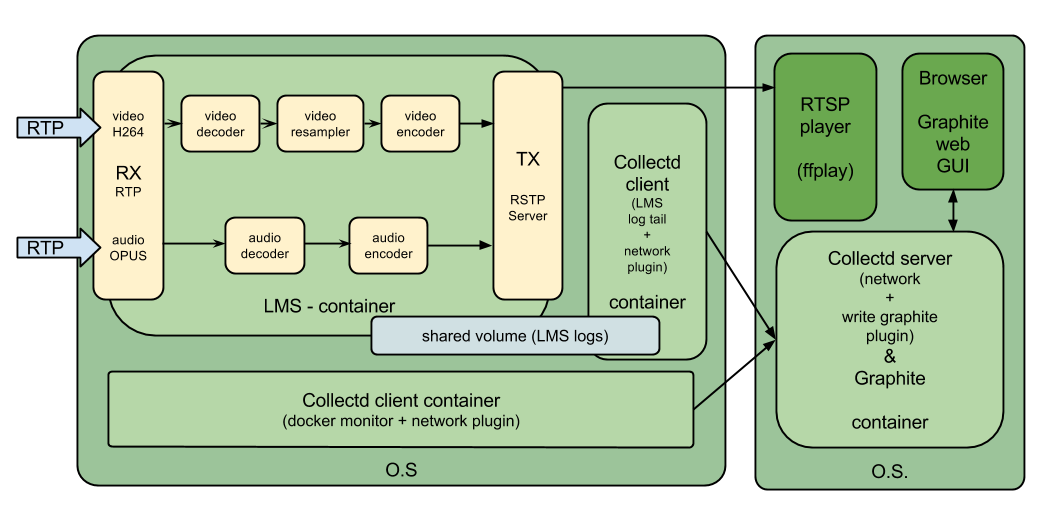
\includegraphics[width=0.95\textwidth]{./images/isolatedScenario.png}
\caption{Isolated demonstration's scenario configuration}
\label{F:idsc}
\end{center}
\end{figure}

The Collectd client container, which reads from the volume where the LMS container is logging its metrics, is using the \texttt{tail} plugin (previously explained in chapter \ref{G:monitoringLayer}) with specific regular expressions in order to parse the metrics from the LMS logs.

So, both isolated scenarios are the same but one is running the LMS on the system and the other is running the same configured LMS but containerized.

The second OS running is the one which runs the Docker container with the Collectd+Graphite tools. Moreover, this OS acts as the receiver of the transcoded streams through RTSP protocol and also as the transmitter of the source stream.

Therefore, in figure \ref{F:isoCPU} the results of interest are shown and grouped. These are mainly focused on the pipeline performance metrics (i.e.: internal LMS performance).

\begin{figure}[!htb]
  \begin{center}
    \begin{subfigmatrix}{2}
      \subfigure[System installation]
         {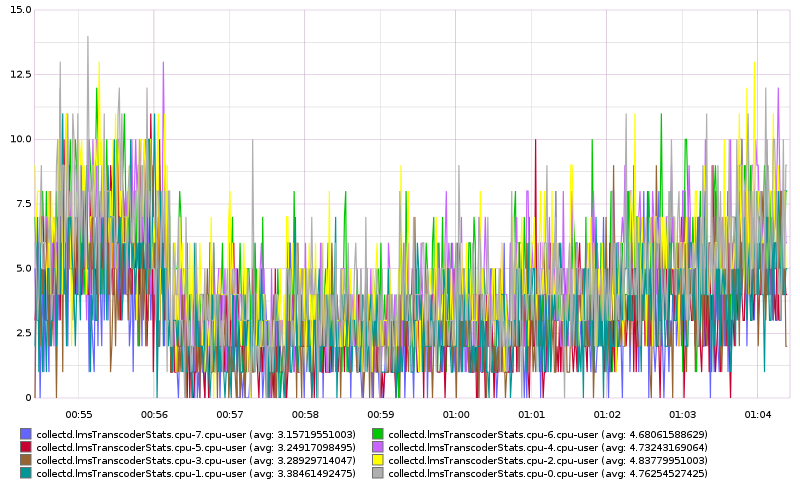
\includegraphics{./images/testStats/testStatsOS/8cpuIdleAVG.png}\label{SF:S1}} 
      \subfigure[Containerized]
         {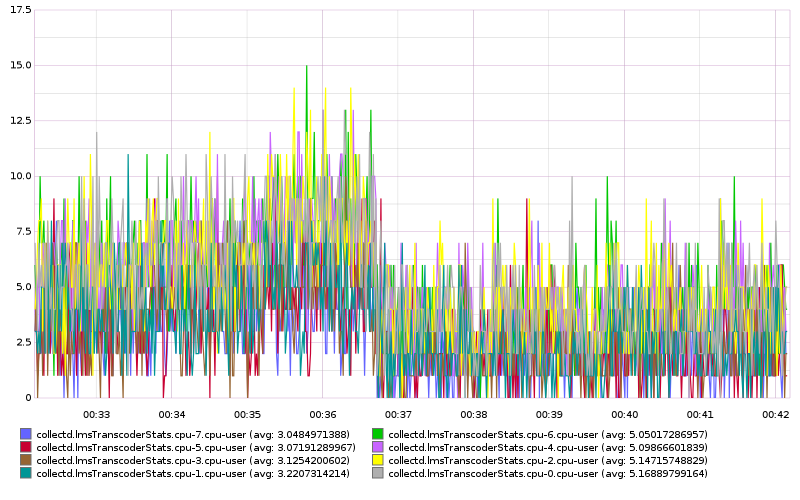
\includegraphics{./images/testStats/testStatsDocker/8cpuIdleAVG.png}\label{SF:S2}} 
    \end{subfigmatrix}
    \caption{Isolated scenarios - CPU usage}
    \label{F:isoCPU}
  \end{center}
\end{figure}

Figure \ref{F:isoCPU} showcases the CPU usage gathered at the Collectd client side and presented for the Graphite web GUI for both isolated scenarios. Regarding system installation the CPU average usage of the averages given by Graphite is around 4,015\% and around 4,111\% for the containerized one. So, there is not so difference about running system installation or the same application containerized. 

In order to continue demonstrating that the fact of deploying a service platform within a containerized environment figure \ref{F:isoappt} is showcasing results of interest.

\begin{figure}[!htb]
  \begin{center}
    \begin{subfigmatrix}{2}
      \subfigure[System installation - Video path]
         {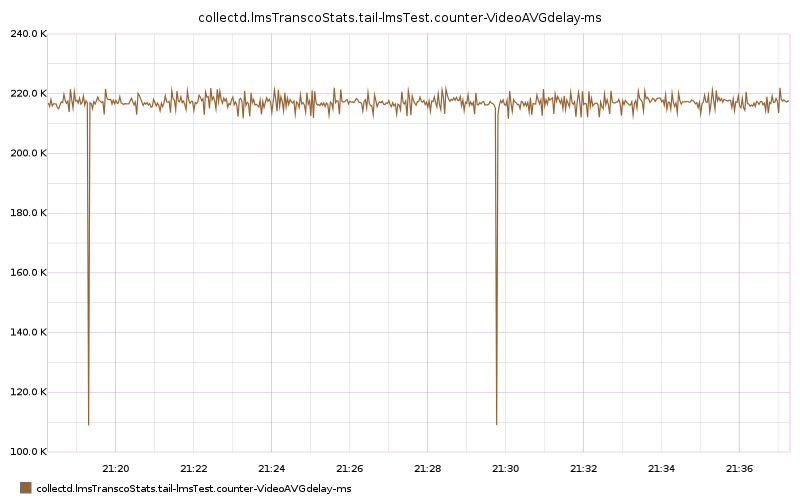
\includegraphics{./images/testStats/testStatsOS/vAVGdelayMS.png}\label{SF:S3}} 
      \subfigure[Containerized - Video path]
         {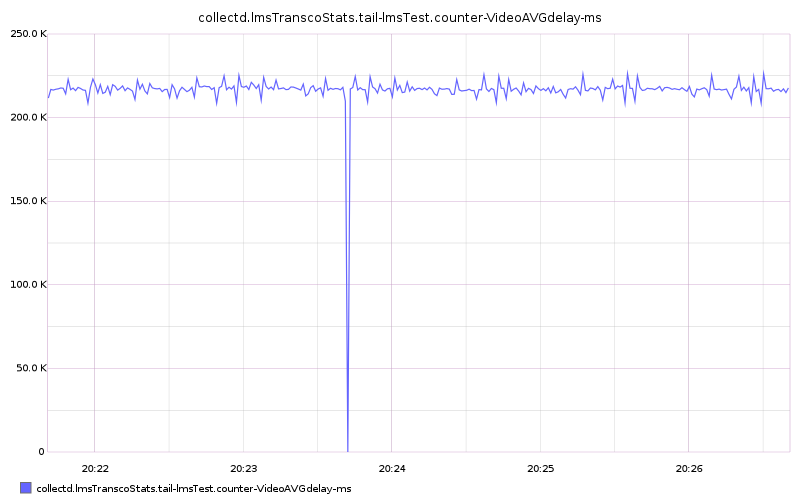
\includegraphics{./images/testStats/testStatsDocker/vAVGdelayMS.png}\label{SF:S4}} 
      \subfigure[System installation - Audio path]
         {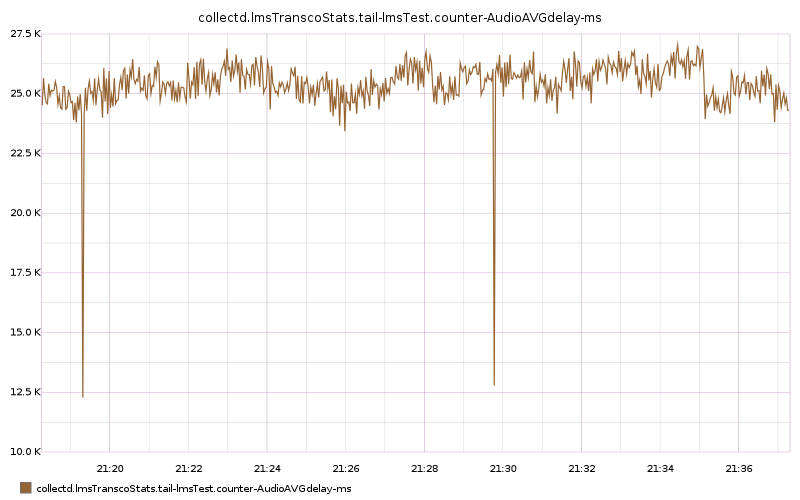
\includegraphics{./images/testStats/testStatsOS/aAVGdelayMS.png}\label{SF:S3}} 
      \subfigure[Containerized - Audio path]
         {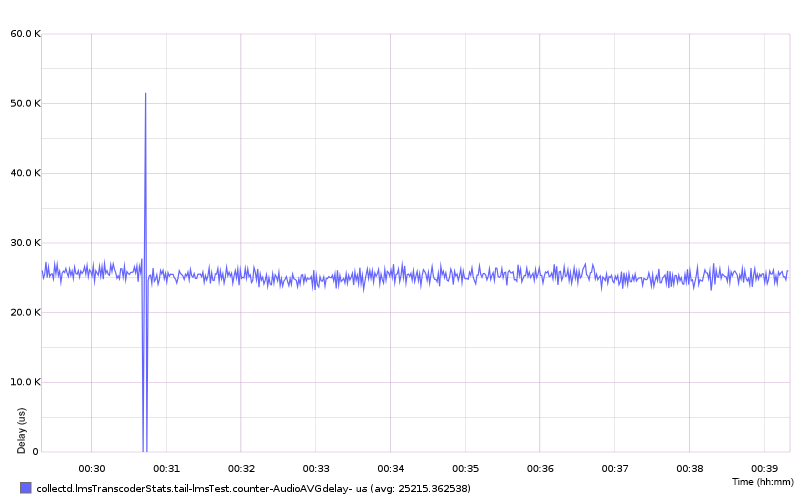
\includegraphics{./images/testStats/testStatsDocker/aAVGdelayMS.png}\label{SF:S4}}
    \end{subfigmatrix}
    \caption{Isolated scenarios - average pipeline processing time}
    \label{F:isoappt}
  \end{center}
\end{figure}

Figure \ref{F:isoappt} showcases the average pipelines delay introduced for the LMS system which in both video and audio cases is almost the same. Regarding the video, system installation reaches an average of 216,8 milliseconds and the containerized reaches an average of 215,9 milliseconds. Then, regarding audio system installation reaches an average of 25,6 milliseconds and the containerized reaches an average of 25,2 milliseconds.

\begin{figure}[!htb]
  \begin{center}
    \begin{subfigmatrix}{2}
      \subfigure[System installation - Video path]
         {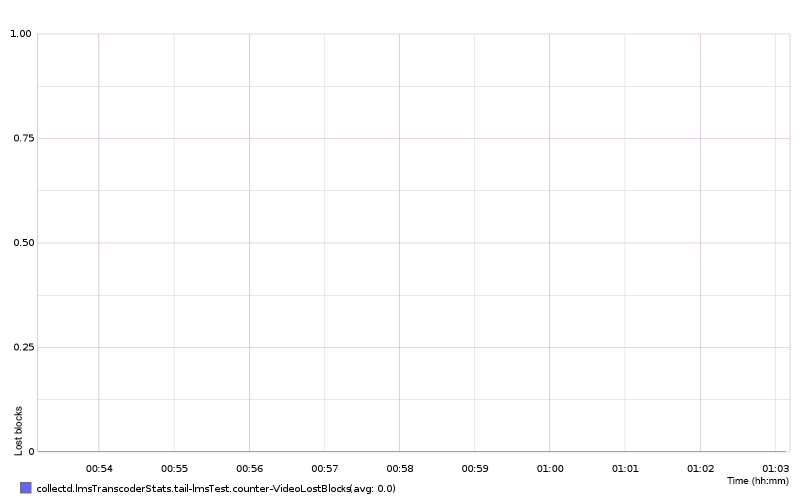
\includegraphics{./images/testStats/testStatsOS/vLostBlocs.png}\label{SF:S3}} 
      \subfigure[Containerized - Video path]
         {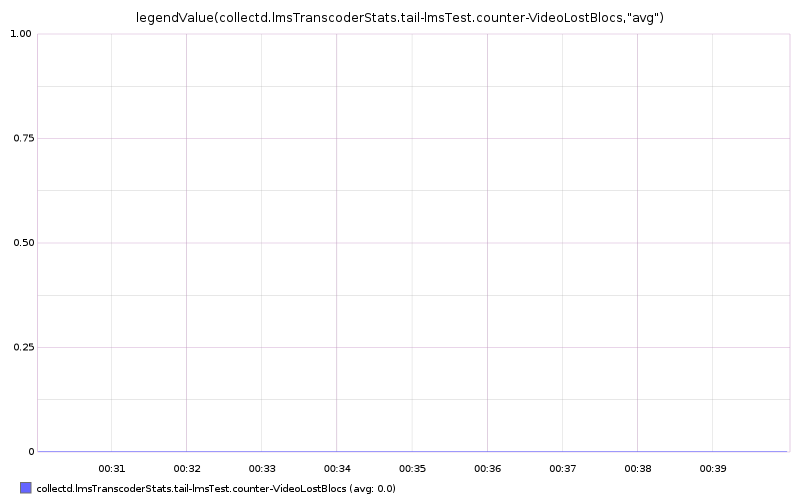
\includegraphics{./images/testStats/testStatsDocker/vLostBlocs.png}\label{SF:S4}} 
      \subfigure[System installation - Audio path]
         {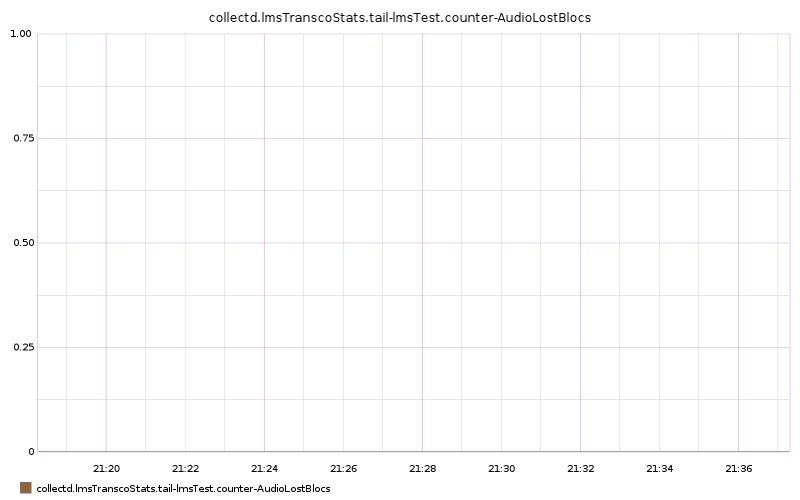
\includegraphics{./images/testStats/testStatsOS/aLostBlocs.png}\label{SF:S3}} 
      \subfigure[Containerized - Audio path]
         {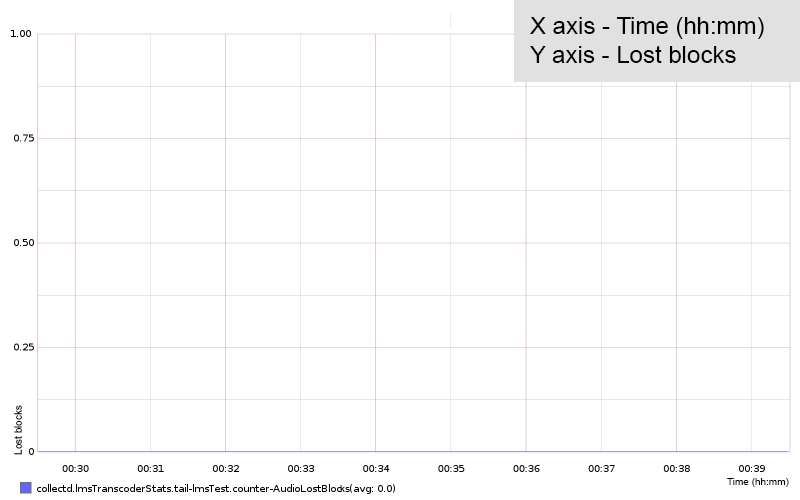
\includegraphics{./images/testStats/testStatsDocker/aLostBlocs.png}\label{SF:S4}}
    \end{subfigmatrix}
    \caption{Isolated scenarios - pipeline accumulated lost blocs}
    \label{F:isoaplb}
  \end{center}
\end{figure} 

Regarding pipeline losses, as shown in figure \ref{F:isoaplb} both pipelines within both system installation and containerized scenarios don't introduce any data loss.

And this is a sign that LMS is a good option to work with not only on system installation but in a containerized environment in order to be a portable service over a cloud infrastructure.

\subsection{Generic scenario demonstration}

This last scenario aims to be a generic and basic example demonstration of audio and video production in a cloud environment. Figure \ref{F:gdsc} showcases how the scenario is configured.

\begin{figure}[htb]
\begin{center}
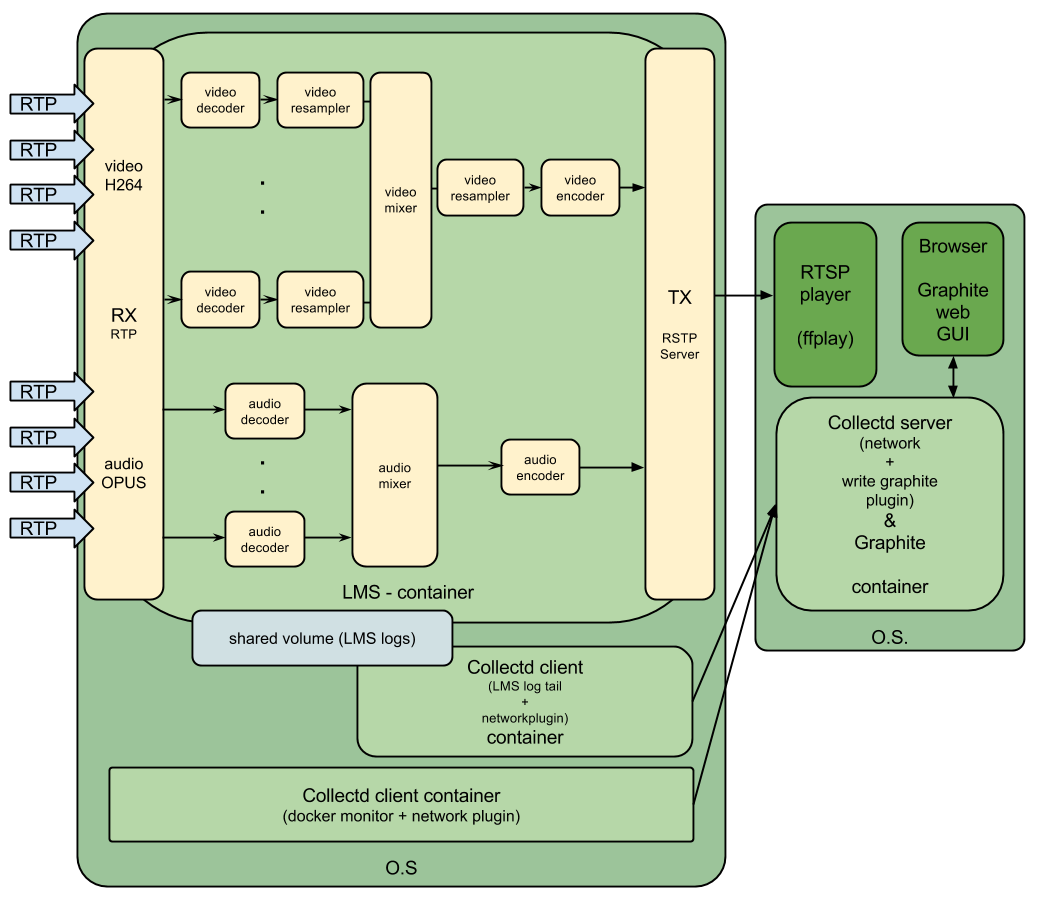
\includegraphics[width=0.95\textwidth]{./images/genericScenario.png}
\caption{Generic demonstration's scenario configuration}
\label{F:gdsc}
\end{center}
\end{figure}

This demonstration is quite similar than the other but this time LMS is only configured and running inside a container. This LMS configuration is also a C/C++ script which congiures the framework, as shown in figure \ref{F:gdsc}, inside the LMS container, specifically.

So, in this case what is deployed is an audio and video mixer which receives four audio streams and four video streams encoded with OPUS and H264 codecs, respectively, which are streamed through its standard RTP encapsulation (i.e.: specific payload headers).

Regarding the audio mixing, all input streams are mixed with logarithmic mixing algorithm in order to not saturate the signal of the resulting audio stream. Then, regarding the video mixing, the HD inputs (i.e.: 1280x720 pixels of resolution) are mixed as shown in figure \ref{F:outVMix}.

\begin{figure}[!htb]
\begin{center}
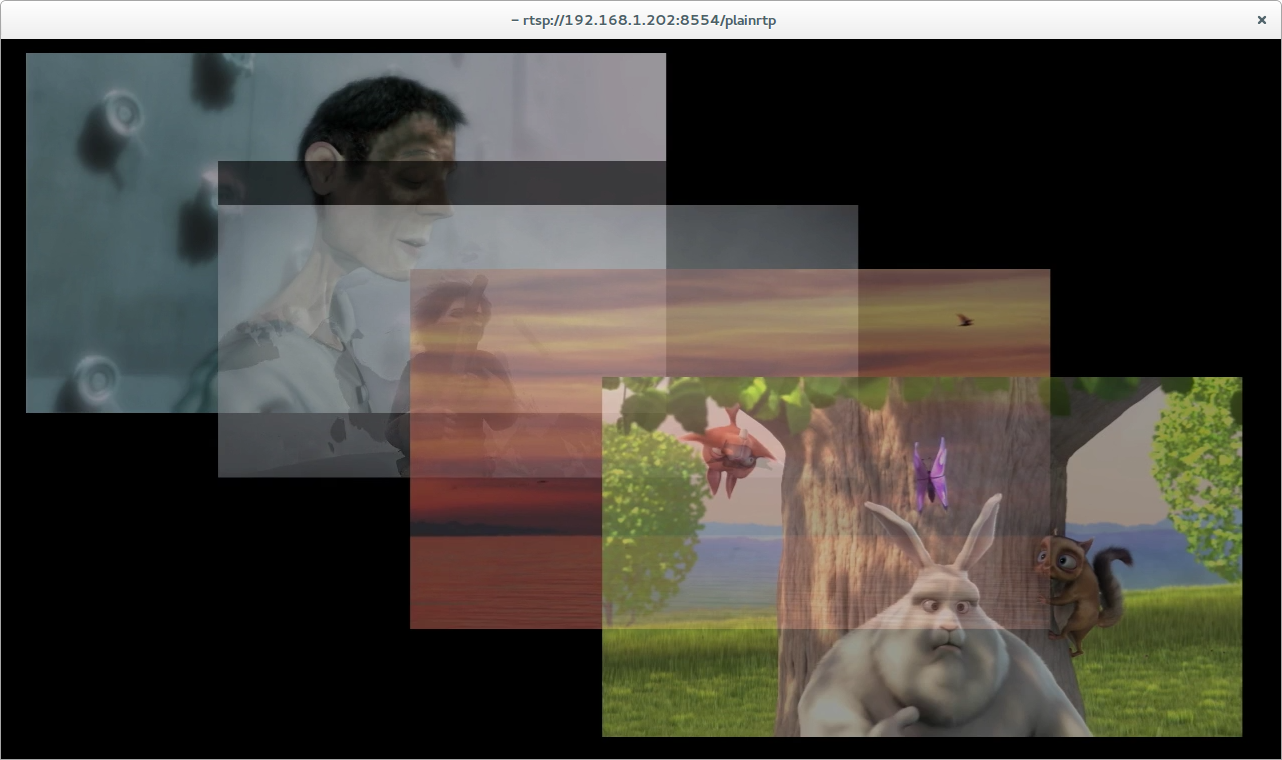
\includegraphics[width=0.90\textwidth]{./images/outAVmix.png}
\caption{Generic scenario - video mixing configuration result}
\label{F:outVMix}
\end{center}
\end{figure}

All video inputs are resized (through the pre-resampler filter to the video mixer, see \ref{F:gdsc}) to the half of its size in order to fill into a resulting HD video stream as shown in figure \ref{F:gdsc}.

So, once the scenario is introduced, let's focus on the obtained results of interest as done in previous section. This is focusing on the pipeline performance parameters.

The CPU usage of the containerized audio and video mixer obtained by averaging the averages shown in figure \ref{F:gsavgcpu} is about the 23,02\%.

\begin{figure}[!htb]
\begin{center}
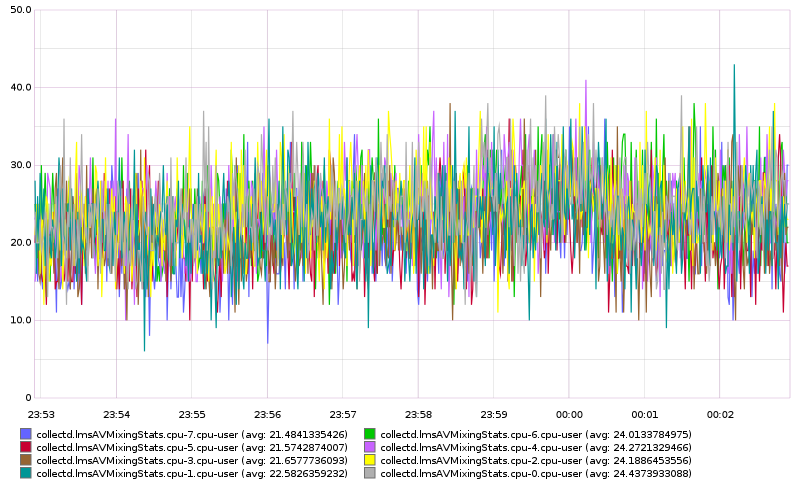
\includegraphics[width=0.90\textwidth]{./images/testAVMix/AVMixCPU.png}
\caption{Generic scenario - average CPU usage}
\label{F:gsavgcpu}
\end{center}
\end{figure}

Then,the audio and video average pipeline delay introduced for this scenario's configuration is as shown in figure \ref{F:gsavgpt}. There are two path groups, the "recevier to mixer" paths and the "mixer to transmitter" path (see figure \ref{F:gdsc}).

\begin{figure}[!htb]
  \begin{center}
    \begin{subfigmatrix}{2}
      \subfigure[Audio paths]
         {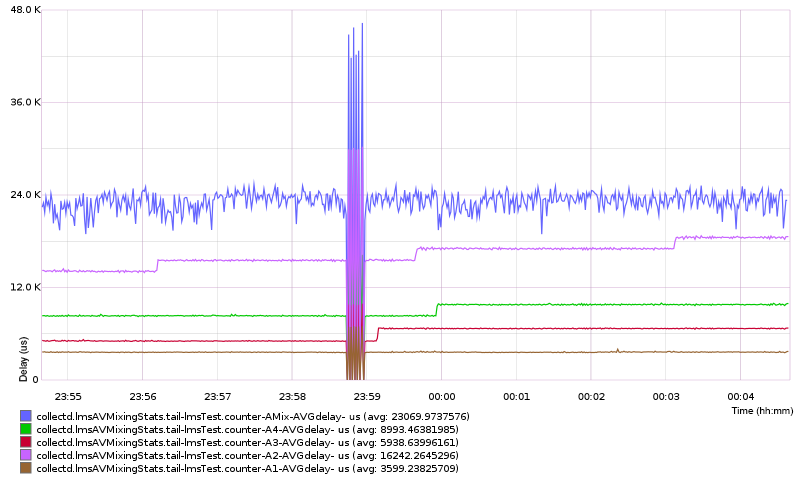
\includegraphics{./images/testAVMix/AVMixAudioAVGdelay.png}\label{SF:S5}} 
      \subfigure[Video paths]
         {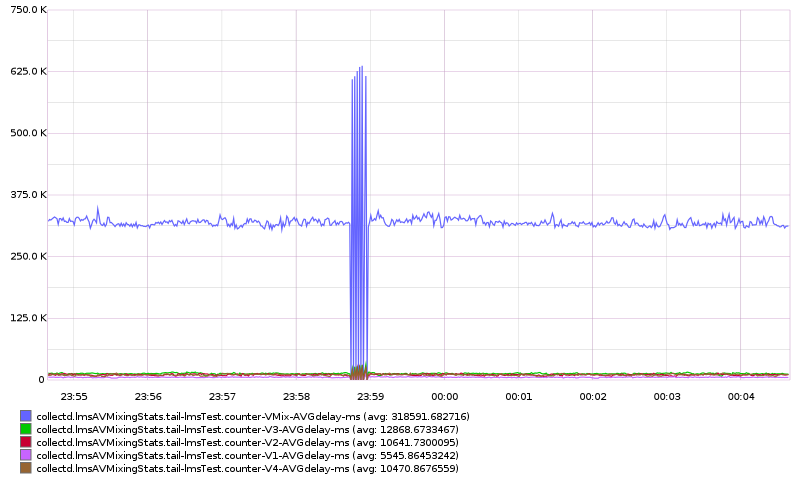
\includegraphics{./images/testAVMix/AVMixVideoAVGdelay.png}\label{SF:S6}} 
    \end{subfigmatrix}
    \caption{Generic scenario - paths average processing time}
    \label{F:gsavgpt}
  \end{center}
\end{figure}

So, the average delay introduced for the audio "receiver to mixer" paths averages is about 8,6 milliseconds and the audio "mixer to transmitter" path average delay is about 23.1 milliseconds. Then, by adding the maximum average path (16,2), a total average value of 39,3 milliseconds of average processing time regarding the audio pipeline is achieved. Then, regarding the same calculus but about the video pipeline path's, an average of 9,89 milliseconds is obtained by averaging the "receiver to mixer" video paths average processing times. And, by adding the average of the "mixer to transmitter" path processing time of 67 milliseconds to the maximum average obtained in the "receiver to mixer" path (12,8 ms) a total average of 79,8 milliseconds of delay introduced for the video pipeline is obtained.

\begin{figure}[!htb]
  \begin{center}
    \begin{subfigmatrix}{2}
      \subfigure[Audio paths]
         {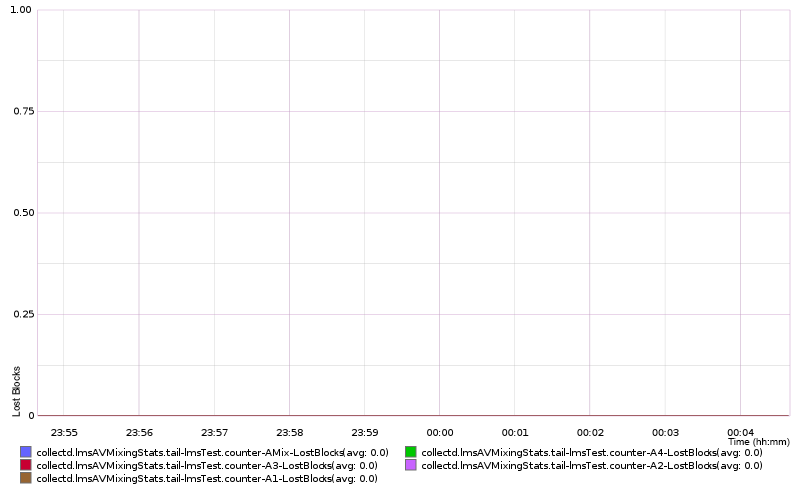
\includegraphics{./images/testAVMix/AVMixAudioLostBlocs.png}\label{SF:S7}} 
      \subfigure[Video paths]
         {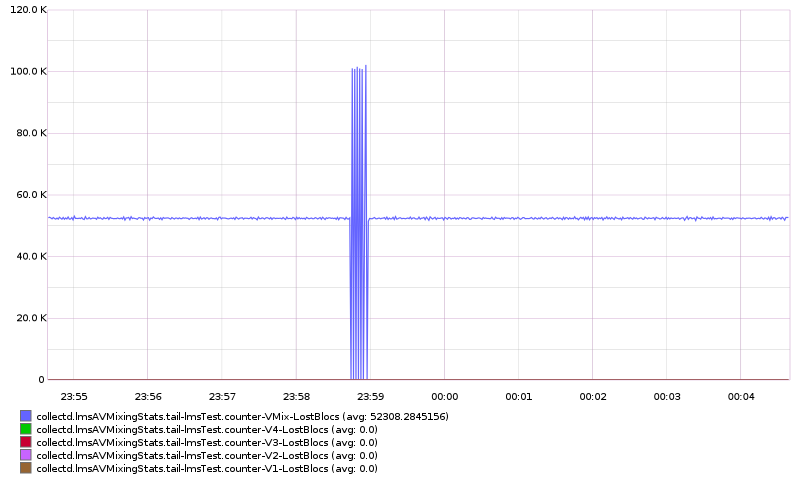
\includegraphics{./images/testAVMix/AVMixVideoLostBlocs.png}\label{SF:S8}} 
    \end{subfigmatrix}
    \caption{Generic scenario - paths accumulated lost blocs}
    \label{F:gsalb}
  \end{center}
\end{figure}

In figure \ref{F:gsalb} the audio paths accumulated lost blocs remains to zero meaning that the audio pipeline is not discarding any data at any filter, which is an important fact because losing any byte of audio means hearing it. 

Then regarding the video "receiver to mixer" paths there aren't accumulated data losses. But, "mixer to transmitter" path reaches around 52.308 lost data blocs. The fact of having lost data blocs is due to the transitory period of the mixer filter. However, this accumulated losses remains constant, meaning that there are no more data blocs lost.

So, although this scenario is being deployed in a i7 processor laptop, it's able to real-time mix four couples of audio and video streams without issues.

Finally, to point out that the appearing burst in some figures are due to the fact of transmitting origin streams in a pseudo-live mode, which means audio and video loops. Therefore, these bursts appear when restarting the origin streams.